\documentclass[a4paper]{article}

\def\npart {IV}
\def\nterm {Michaelmas}
\def\nyear {2017}
\def\nlecturer {H.\ Wilton}
\def\ncourse {Topics in Geometric Group Theory}

% Imports
\ifx \nextra \undefined
  \usepackage[pdftex,
    hidelinks,
    pdfauthor={Dexter Chua},
    pdfsubject={Cambridge Maths Notes: Part \npart\ - \ncourse},
    pdftitle={Part \npart\ - \ncourse},
  pdfkeywords={Cambridge Mathematics Maths Math \npart\ \nterm\ \nyear\ \ncourse}]{hyperref}
  \title{Part \npart\ - \ncourse}
\else
  \usepackage[pdftex,
    hidelinks,
    pdfauthor={Dexter Chua},
    pdfsubject={Cambridge Maths Notes: Part \npart\ - \ncourse\ (\nextra)},
    pdftitle={Part \npart\ - \ncourse\ (\nextra)},
  pdfkeywords={Cambridge Mathematics Maths Math \npart\ \nterm\ \nyear\ \ncourse\ \nextra}]{hyperref}

  \title{Part \npart\ - \ncourse \\ {\Large \nextra}}
\fi

\author{Lectured by \nlecturer \\\small Notes taken by Dexter Chua}
\date{\nterm\ \nyear}

\usepackage{alltt}
\usepackage{amsfonts}
\usepackage{amsmath}
\usepackage{amssymb}
\usepackage{amsthm}
\usepackage{booktabs}
\usepackage{caption}
\usepackage{enumitem}
\usepackage{fancyhdr}
\usepackage{graphicx}
\usepackage{mathtools}
\usepackage{microtype}
\usepackage{multirow}
\usepackage{pdflscape}
\usepackage{pgfplots}
\usepackage{siunitx}
\usepackage{tabularx}
\usepackage{tikz}
\usepackage{tkz-euclide}
\usepackage[normalem]{ulem}
\usepackage[all]{xy}

\pgfplotsset{compat=1.12}

\pagestyle{fancyplain}
\lhead{\emph{\nouppercase{\leftmark}}}
\ifx \nextra \undefined
  \rhead{
    \ifnum\thepage=1
    \else
      \npart\ \ncourse
    \fi}
\else
  \rhead{
    \ifnum\thepage=1
    \else
      \npart\ \ncourse\ (\nextra)
    \fi}
\fi
\usetikzlibrary{arrows}
\usetikzlibrary{decorations.markings}
\usetikzlibrary{decorations.pathmorphing}
\usetikzlibrary{positioning}
\usetikzlibrary{fadings}
\usetikzlibrary{intersections}
\usetikzlibrary{cd}

\newcommand*{\Cdot}{\raisebox{-0.25ex}{\scalebox{1.5}{$\cdot$}}}
\newcommand {\pd}[2][ ]{
  \ifx #1 { }
    \frac{\partial}{\partial #2}
  \else
    \frac{\partial^{#1}}{\partial #2^{#1}}
  \fi
}

% Theorems
\theoremstyle{definition}
\newtheorem*{aim}{Aim}
\newtheorem*{axiom}{Axiom}
\newtheorem*{claim}{Claim}
\newtheorem*{cor}{Corollary}
\newtheorem*{defi}{Definition}
\newtheorem*{eg}{Example}
\newtheorem*{fact}{Fact}
\newtheorem*{law}{Law}
\newtheorem*{lemma}{Lemma}
\newtheorem*{notation}{Notation}
\newtheorem*{prop}{Proposition}
\newtheorem*{thm}{Theorem}

\renewcommand{\labelitemi}{--}
\renewcommand{\labelitemii}{$\circ$}
\renewcommand{\labelenumi}{(\roman{*})}

\let\stdsection\section
\renewcommand\section{\newpage\stdsection}

% Strike through
\def\st{\bgroup \ULdepth=-.55ex \ULset}

% Maths symbols
\newcommand{\bra}{\langle}
\newcommand{\ket}{\rangle}

\newcommand{\N}{\mathbb{N}}
\newcommand{\Z}{\mathbb{Z}}
\newcommand{\Q}{\mathbb{Q}}
\renewcommand{\H}{\mathbb{H}}
\newcommand{\R}{\mathbb{R}}
\newcommand{\C}{\mathbb{C}}
\newcommand{\Prob}{\mathbb{P}}
\renewcommand{\P}{\mathbb{P}}
\newcommand{\E}{\mathbb{E}}
\newcommand{\F}{\mathbb{F}}
\newcommand{\cU}{\mathcal{U}}
\newcommand{\RP}{\mathbb{RP}}
\newcommand{\CP}{\mathbb{CP}}

\newcommand{\ph}{\,\cdot\,}

\DeclareMathOperator{\sech}{sech}
\DeclareMathOperator{\cosech}{cosech}
\DeclareMathOperator{\cosec}{cosec}

\DeclareMathOperator{\covol}{covol}
\DeclareMathOperator{\vol}{vol}

\let\Im\relax
\let\Re\relax
\DeclareMathOperator{\Im}{Im}
\DeclareMathOperator{\Re}{Re}
\DeclareMathOperator{\im}{im}
\DeclareMathOperator{\image}{image}
\DeclareMathOperator{\Ann}{Ann}

\DeclareMathOperator*{\res}{res}
\DeclareMathOperator{\Res}{Res}
\DeclareMathOperator{\Ind}{Ind}

\DeclareMathOperator{\tr}{tr}
\DeclareMathOperator{\diag}{diag}
\DeclareMathOperator{\rank}{rank}
\DeclareMathOperator{\card}{card}
\DeclareMathOperator{\spn}{span}
\DeclareMathOperator{\adj}{adj}

\DeclareMathOperator{\erf}{erf}
\DeclareMathOperator{\erfc}{erfc}

\DeclareMathOperator{\ord}{ord}
\DeclareMathOperator{\Sym}{Sym}

\DeclareMathOperator{\sgn}{sgn}
\DeclareMathOperator{\orb}{orb}
\DeclareMathOperator{\stab}{stab}
\DeclareMathOperator{\ccl}{ccl}

\DeclareMathOperator{\lcm}{lcm}
\DeclareMathOperator{\hcf}{hcf}

\DeclareMathOperator{\Int}{Int}
\DeclareMathOperator{\id}{id}

\DeclareMathOperator{\betaD}{beta}
\DeclareMathOperator{\gammaD}{gamma}
\DeclareMathOperator{\Poisson}{Poisson}
\DeclareMathOperator{\binomial}{binomial}
\DeclareMathOperator{\multinomial}{multinomial}
\DeclareMathOperator{\Bernoulli}{Bernoulli}
\DeclareMathOperator{\like}{like}

\DeclareMathOperator{\var}{var}
\DeclareMathOperator{\cov}{cov}
\DeclareMathOperator{\bias}{bias}
\DeclareMathOperator{\mse}{mse}
\DeclareMathOperator{\corr}{corr}

\DeclareMathOperator{\otp}{otp}
\DeclareMathOperator{\dom}{dom}

\DeclareMathOperator{\Root}{Root}
\DeclareMathOperator{\supp}{supp}
\DeclareMathOperator{\rel}{rel}
\DeclareMathOperator{\Hom}{Hom}
\DeclareMathOperator{\Aut}{Aut}
\DeclareMathOperator{\Gal}{Gal}
\DeclareMathOperator{\Mat}{Mat}
\DeclareMathOperator{\End}{End}
\DeclareMathOperator{\Char}{char}
\DeclareMathOperator{\ev}{ev}
\DeclareMathOperator{\St}{St}
\DeclareMathOperator{\Lk}{Lk}
\DeclareMathOperator{\disc}{disc}
\DeclareMathOperator{\Isom}{Isom}
\DeclareMathOperator{\length}{length}
\DeclareMathOperator{\energy}{energy}
\DeclareMathOperator{\area}{area}
\DeclareMathOperator{\Syl}{Syl}
\DeclareMathOperator{\cl}{cl}
\DeclareMathOperator{\fix}{fix}

\newcommand{\GL}{\mathrm{GL}}
\newcommand{\SL}{\mathrm{SL}}
\newcommand{\PGL}{\mathrm{PGL}}
\newcommand{\PSL}{\mathrm{PSL}}
\newcommand{\PSU}{\mathrm{PSU}}
\newcommand{\Or}{\mathrm{O}}
\newcommand{\SO}{\mathrm{SO}}
\newcommand{\U}{\mathrm{U}}
\newcommand{\SU}{\mathrm{SU}}

\renewcommand{\d}{\mathrm{d}}
\newcommand{\D}{\mathrm{D}}

\tikzset{->/.style = {decoration={markings,
                                  mark=at position 1 with {\arrow[scale=2]{latex'}}},
                      postaction={decorate}}}
\tikzset{<-/.style = {decoration={markings,
                                  mark=at position 0 with {\arrowreversed[scale=2]{latex'}}},
                      postaction={decorate}}}
\tikzset{<->/.style = {decoration={markings,
                                   mark=at position 0 with {\arrowreversed[scale=2]{latex'}},
                                   mark=at position 1 with {\arrow[scale=2]{latex'}}},
                       postaction={decorate}}}
\tikzset{->-/.style = {decoration={markings,
                                   mark=at position #1 with {\arrow[scale=2]{latex'}}},
                       postaction={decorate}}}
\tikzset{-<-/.style = {decoration={markings,
                                   mark=at position #1 with {\arrowreversed[scale=2]{latex'}}},
                       postaction={decorate}}}

\tikzset{circ/.style = {fill, circle, inner sep = 0, minimum size = 3}}
\tikzset{mstate/.style={circle, draw, blue, text=black, minimum width=0.7cm}}

\definecolor{mblue}{rgb}{0.2, 0.3, 0.8}
\definecolor{morange}{rgb}{1, 0.5, 0}
\definecolor{mgreen}{rgb}{0.1, 0.4, 0.2}
\definecolor{mred}{rgb}{0.5, 0, 0}

\def\drawcirculararc(#1,#2)(#3,#4)(#5,#6){%
    \pgfmathsetmacro\cA{(#1*#1+#2*#2-#3*#3-#4*#4)/2}%
    \pgfmathsetmacro\cB{(#1*#1+#2*#2-#5*#5-#6*#6)/2}%
    \pgfmathsetmacro\cy{(\cB*(#1-#3)-\cA*(#1-#5))/%
                        ((#2-#6)*(#1-#3)-(#2-#4)*(#1-#5))}%
    \pgfmathsetmacro\cx{(\cA-\cy*(#2-#4))/(#1-#3)}%
    \pgfmathsetmacro\cr{sqrt((#1-\cx)*(#1-\cx)+(#2-\cy)*(#2-\cy))}%
    \pgfmathsetmacro\cA{atan2(#2-\cy,#1-\cx)}%
    \pgfmathsetmacro\cB{atan2(#6-\cy,#5-\cx)}%
    \pgfmathparse{\cB<\cA}%
    \ifnum\pgfmathresult=1
        \pgfmathsetmacro\cB{\cB+360}%
    \fi
    \draw (#1,#2) arc (\cA:\cB:\cr);%
}
\newcommand\getCoord[3]{\newdimen{#1}\newdimen{#2}\pgfextractx{#1}{\pgfpointanchor{#3}{center}}\pgfextracty{#2}{\pgfpointanchor{#3}{center}}}

\def\Xint#1{\mathchoice
   {\XXint\displaystyle\textstyle{#1}}%
   {\XXint\textstyle\scriptstyle{#1}}%
   {\XXint\scriptstyle\scriptscriptstyle{#1}}%
   {\XXint\scriptscriptstyle\scriptscriptstyle{#1}}%
   \!\int}
\def\XXint#1#2#3{{\setbox0=\hbox{$#1{#2#3}{\int}$}
     \vcenter{\hbox{$#2#3$}}\kern-.5\wd0}}
\def\ddashint{\Xint=}
\def\dashint{\Xint-}


\newcommand\Cay{\mathrm{Cay}}
%\newcommand\qi{\underset{qi}{\simeq}}
\newcommand{\qi}{\underset{qi}{\simeq}}

\begin{document}
\maketitle
{\small
\setlength{\parindent}{0em}
\setlength{\parskip}{1em}

The subject of geometric group theory is founded on the observation that the algebraic and algorithmic properties of a discrete group are closely related to the geometric features of the spaces on which the group acts. This graduate course will provide an introduction to the basic ideas of the subject.

Suppose $\Gamma$ is a discrete group of isometries of a metric space $X$. We focus on the theorems we can prove about $\Gamma$ by imposing geometric conditions on $X$. These conditions are motivated by curvature conditions in differential geometry, but apply to general metric spaces and are much easier to state. First we study the case when $X$ is \emph{Gromov-hyperbolic}, which corresponds to negative curvature. Then we study the case when $X$ is \emph{CAT(0)}, which corresponds to non-positive curvature. In order for this theory to be useful, we need a rich supply of negatively and non-positively curved spaces. We develop the theory of \emph{non-positively curved cube complexes}, which provide many examples of CAT(0) spaces and have been the source of some dramatic developments in low-dimensional topology over the last twenty years.

\begin{itemize}
 \item[Part 1.] We will introduce the basic notions of geometric group theory: Cayley graphs, quasiisometries, the Schwarz--Milnor Lemma, and the connection with algebraic topology via presentation complexes. We will discuss the word problem, which is quantified using the Dehn functions of a group.
 \item[Part 2.] We will cover the basic theory of word-hyperbolic groups, including the Morse lemma, local characterization of quasigeodesics, linear isoperimetric inequality, finitely presentedness, quasiconvex subgroups etc.
 \item[Part 3.] We will cover the basic theory of CAT(0) spaces, working up to the Cartan--Hadamard theorem and Gromov's Link Condition. These two results together enable us to check whether the universal cover of a complex admits a CAT(1) metric.
 \item[Part 4.] We will introduce cube complexes, in which Gromov's link condition becomes purely combinatorial. If there is time, we will discuss Haglund--Wise's \emph{special} cube complexes, which combine the good geometric properties of CAT(0) spaces with some strong algebraic and topological properties
\end{itemize}

\subsubsection*{Pre-requisites}
Part IB Geometry and Part II Algebraic topology are required.
}

\tableofcontents

\section{Cayley graphs and the word metric}
There is this unfortunate tendency for people to think of groups as being part of algebra. Which is, perhaps, reasonable. There are elements and there are operations on them. These operations satisfy some algebraic laws. But there is also geometry involved. For example, one of the simplest non-abelian groups we know is $D_6$, the group of symmetries of a triangle. This is fundamentally a geometric idea, and often this geometric interpretation can let us prove a lot of things about $D_6$.

In general, the way we find groups in nature is that we have some object, and we look at its symmetry. In geometric group theory, what we do is that we want to remember the object the group acts on, and often these objects have some geometric structure. In fact, we shall see that all groups are symmetries of some geometric object.

Let $\Gamma$ be a group, and $S$ a generating set for $\Gamma$. For the purposes of this course, $S$ will be finite. So in this course, we are mostly going to think about finitely-generated groups. Of course, there are non-finitely-generated groups out there in the wild, but we will have to put in some more effort to make our ideas work.

The simplest geometric idea we can think of is that of distance, i.e.\ a metric. So we want to use our generating set $S$ to make $G$ into a metric space.

\begin{defi}[Word length]\index{word length}
  Let $\Gamma$ be a group and $S$ a finite generating set. If $\gamma \in \Gamma$, the \emph{word length} of $\gamma$ is
  \[
    \ell_S(\gamma) = \min \{n : \gamma = s_1^{\pm 1} \cdots s_n^{\pm 1}\text{ for some } s_i \in S\}.
  \]
\end{defi}

\begin{defi}[Word metric]\index{word metric}
  Let $\Gamma$ be a group and $S$ a finite generating set. The \emph{word metric} on $\Gamma$ is given by
  \[
    d_S (\gamma_1, \gamma_2) = \ell_s(\gamma_1^{-1} \gamma_2).
  \]
\end{defi}

If we stare at the definition, we see that the word metric is left-invariant, i.e.\ for any $g, \gamma_1, \gamma_2 \in \Gamma$, we have
\[
  d_S(g \gamma_1, g \gamma_2) = d_S(\gamma_1, \gamma_2).
  \]
However, it is usually not the case that the metric is right invariant, i.e.\ $d_S(\gamma_1 g, \gamma_2 g)$ is not equal to $d_S(\gamma_1, \gamma_2)$. This is one of the prices we have to pay for wanting to do geometry.

If we tried to draw our metric space out, it looks pretty unhelpful --- it's just a bunch of dots. It is not path connected. We can't really think about it well. The solution is provided by Cayley graphs.

\begin{defi}[Cayley graph]\index{Cayley graph}
  The \emph{Cayley graph} $\Cay_S(G)$ is defined as follows:
  \begin{itemize}
    \item $V(\Cay_S(\Gamma)) = \Gamma$
    \item For each $\gamma \in G$ and $s \in S$, we draw an edge from $\gamma$ to $\gamma s$.
  \end{itemize}
\end{defi}
If we want it to be a directed and labelled graph, we can label the edge by the generator $s$.

How does this relate to the word metric? There is an obvious left action of $\Gamma$ on $\Cay_S(\Gamma)$ which extends the left action of $\Gamma$ on itself. This is since the edge is defined by multiplication of the generator on the \emph{right}.

Moreover the word metric on $\Gamma$ extends to a metric on $\Cay_S(\Gamma)$ in which every edge is isometric to $[0, 1]$.

Finally, note that $\Cay_S(\Gamma)$ is always regular, where the degree of each vertex is $2|S|$.

\begin{eg}
  Take $\Gamma = C_2 = \Z/2\Z$, and take $S = \{1\}$. Then the Cayley graph looks like
  \begin{center}
    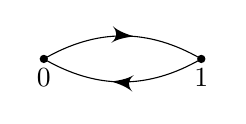
\begin{tikzpicture}
      \node [circ] at (0, 0) {};
      \node [circ] at (2, 0) {};
      \node [below] at (0, 0) {$0$};
      \node [below] at (2, 0) {$1$};

      \draw (0, 0) edge [bend left, ->-=0.57] (2, 0); %insert node saying $1$
      \draw (2, 0) edge [bend left, ->-=0.57] (0, 0);

    \end{tikzpicture}
  \end{center}
\end{eg}

\begin{eg}
  Take $\Gamma = S_3$ and $S = \{(1\; 2), (1\; 2\; 3)\}$. The Cayley graph is
  \begin{center}
    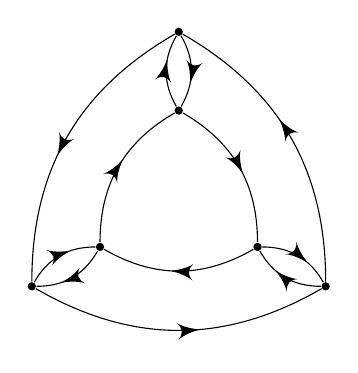
\begin{tikzpicture}
      \node [circ] (L) at (0, 0) {};
      \node [circ] (R) at (2, 0) {};
      \node [circ] (T) at (1, 1.732) {};
      \node [circ] (LL) at (-0.866, -0.5) {};
      \node [circ] (RR) at (2.866, -0.5) {};
      \node [circ] (TT) at (1, 2.732) {}; % this is wrong

%      \node [below] at (L) {$1$};
%      \node at (R) {$(3\; 2\; 1)$};
%      \node at (T) {$(1\; 2\; 3)$};
%      \node at (LL) {$(1\; 2)$};

      \draw (L) edge [bend left, ->-=0.55] (T);
      \draw (T) edge [bend left, ->-=0.55] (R);
      \draw (R) edge [bend left, ->-=0.55] (L);

      \draw (TT) edge [bend right, ->-=0.57] (LL);
      \draw (LL) edge [bend right, ->-=0.57] (RR);
      \draw (RR) edge [bend right, ->-=0.57] (TT);

      \draw (T) edge [bend left, ->-=0.66] (TT);
      \draw (TT) edge [bend left, ->-=0.66] (T);

      \draw (R) edge [bend left, ->-=0.66] (RR);
      \draw (RR) edge [bend left, ->-=0.66] (R);

      \draw (L) edge [bend left, ->-=0.66] (LL);
      \draw (LL) edge [bend left, ->-=0.66] (L);
    \end{tikzpicture}
  \end{center}
\end{eg}

\begin{eg}
  Take $\Gamma = \Z$, and $S = \{1\}$. Then the Cayley graph looks like
  \begin{center}
    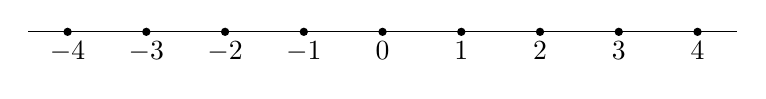
\begin{tikzpicture}
      \foreach \x in {-4,-3,-2,-1,0,1,2,3,4} {
        \node [circ] at (\x, 0) {};
        \node [below] at (\x, 0) {$\x$};
      }
      \draw (-4.5, 0) -- (4.5, 0);
    \end{tikzpicture}
  \end{center}
\end{eg}
\begin{eg}
  Take $\Gamma = \Z$ and $S = \{2, 3\}$. Then the Cayley graph looks like
  \begin{center}
    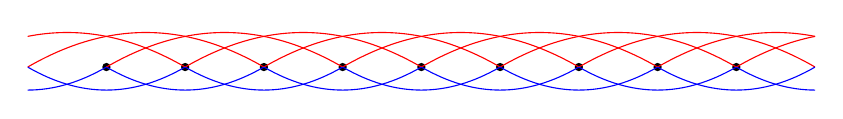
\begin{tikzpicture}
      \clip (-5, -0.3) rectangle (5, 0.5);
      \foreach \x in {-4,-3,-2,-1,0,1,2,3,4} {
        \node [circ] at (\x, 0) {};
      }
      \foreach \x in {-6,-5,-4,-3,-2,-1,0,1,2,3,4} {
        \draw [red] (\x, 0) edge [bend left] +(3, 0);
        \draw [blue] (\x, 0) edge [bend right] +(2, 0);
      }
    \end{tikzpicture}
  \end{center}
\end{eg}
Now this seems quite complicated. It's still the same group $\Gamma = \Z$, but with a different choice of generating set, it looks very different. It seems like what we do depends heavily on the choice of the generating set. 

\begin{eg}
  If $\Gamma = \Z^2$ and $S = \{(1, 0), (0, 1)\}$, then the Cayley graph is a grid
  \begin{center}
    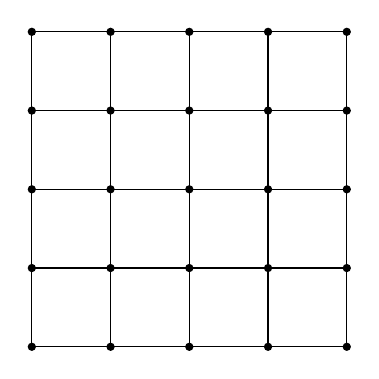
\begin{tikzpicture}
      \foreach \x in {-2,-1,0,1,2} {
        \foreach \y in {-2,-1,0,1,2} {
          \node [circ] at (\x, \y) {};
        }
      }
      \draw [step=1] (-2, -2) grid (2, 2);
    \end{tikzpicture}
  \end{center}
\end{eg}

\begin{eg}
  If $\Gamma = F_2 = \bra a, b\ket$, $S = \{a, b\}$, then the Cayley graph looks like
  \begin{center}
    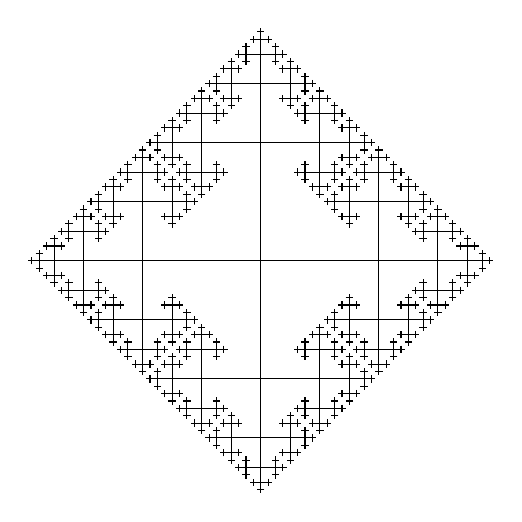
\begin{tikzpicture}[scale=0.5]
      \draw (-3, 0) -- (3, 0);
      \draw (0, -3) -- (0, 3);
      \foreach \x/\y/\rot in {3/0/0, 0/3/90, -3/0/180, 0/-3/270} {
        \begin{scope}[shift={(\x, \y)}, scale=0.5, rotate=\rot]
          \draw (0, 0) -- (3, 0);
          \draw (0, 3) -- (0, -3);
          \foreach \x/\y/\rot in {3/0/0, 0/3/90, 0/-3/270} {
            \begin{scope}[shift={(\x, \y)}, scale=0.5, rotate=\rot]
              \draw (0, 0) -- (3, 0);
              \draw (0, 3) -- (0, -3);
              \foreach \x/\y/\rot in {3/0/0, 0/3/90, 0/-3/270} {
                \begin{scope}[shift={(\x, \y)}, scale=0.5, rotate=\rot]
                  \draw (0, 0) -- (3, 0);
                  \draw (0, 3) -- (0, -3);
                  \foreach \x/\y/\rot in {3/0/0, 0/3/90, 0/-3/270} {
                    \begin{scope}[shift={(\x, \y)}, scale=0.5, rotate=\rot]
                      \draw (0, 0) -- (3, 0);
                      \draw (0, 3) -- (0, -3);
                      \foreach \x/\y/\rot in {3/0/0, 0/3/90, 0/-3/270} {
                        \begin{scope}[shift={(\x, \y)}, scale=0.5, rotate=\rot]
                          \draw (0, 0) -- (3, 0);
                          \draw (0, 3) -- (0, -3);
                        \end{scope}
                      }
                    \end{scope}
                  }
                \end{scope}
              }
            \end{scope}
          }
        \end{scope}
      }
    \end{tikzpicture}
  \end{center}
\end{eg}
If one has done algebraic topology, then one might recognize this as the universal cover of a space. This is not a coincidence, and we will talk about this later.

We now return to the problem we noticed previously. The Cayley graph depends a lot on the generating set chosen, but we want to study the graph without picking a generating set.

What we observe is that while the two Cayley graphs of $\Z$ we drew seem quite different, if we looked at them from $100$ meters away, they look quite similar --- they both look like a long, thin line. This is the idea we are trying to formalize.

\begin{defi}[Quasi-isometry]\index{quasi-isometry}\index{quasi-isometric embedding}
  Let $\lambda \geq 1$ and $c \geq 0$. A function between metric spaces $f: X \to Y$ is a \emph{$(\lambda, c)$-quasi-isometric embedding} if for all $x_1, x_2 \in X$
  \[
    \frac{1}{\lambda} d_X(x_1, x_2) - c \leq d_Y(f(x_1), f(x_2)) \leq \lambda d_X(x,_1, x_2) + c
  \]
  If, in addition, there is a $C$ such that for all $y \in Y$, there exists $x \in X$ such that $d_Y(y, f(x)) \leq C$, we say $f$ is a \emph{quasi-isometry}, and $X$ is \term{quasi-isometric} to $Y$. We write $X\qi Y$.
\end{defi}
The $c$ is saying that we don't care about what happens at scales less than $c$, and the $\lambda$ is just saying we allow ourselves to stretch distances.

Note that if we take $c = 0$, then this is just the notion of a bi-Lipschitz map. But in general, we don't require $f$ to be continuous, since continuity is a rather fine-grained property.

\begin{ex}
  Check that $ X\qi Y$ is an equivalence relation.
\end{ex}
This is not immediately obvious, because there is no inverse to $f$. In fact, we need the axiom of choice to prove this result.

\begin{eg}
  Any bounded metric spaces is quasi-isometric to a point. In particular, if $\Gamma$ is finite, then $(\Gamma, d_S) \qi 1$.
\end{eg}
For this reason, this is not a great point of view for studying finite groups. On the other hand, for infinite groups, this is really useful.

\begin{eg}
  For any $\Gamma$ and $S$, the inclusion $(\Gamma, \Gamma_S)\hookrightarrow (\Cay_S(\Gamma), d_S)$ is a quasi-isometry (take $\lambda = 1, c = 0, C = \frac{1}{2}$).
\end{eg}

The important result is perhaps the following:
\begin{thm}
  For any two finite generating sets $S, S'$ of a group $\Gamma$, the identity map $(\Gamma, d_S) \to (\Gamma, d_{S'})$ is a quasi-isometry.
\end{thm}

\begin{proof}
  Pick
  \[
    \lambda = \max_{s \in S} \ell_{S'}(s),\quad \lambda' \max_{s \in S'} \ell_{S}(s),
  \]
  We then see
  \[
    \ell_S(\gamma) \leq \lambda' \ell_{S'}(\gamma), \quad \ell_{S'}(\gamma) \leq \lambda \ell_s(\gamma). % check
  \]
  for all $\gamma \in \Gamma$. Then the claim follows.
\end{proof}
So as long as we are willing to work up to quasi-isometry, we have a canonically defined geometric object associated to each finitely-generated group.

\begin{defi}[Geodesic]\index{geodesic}
  Let $X$ be a metric space. A \emph{geodesic} in $X$ is an isometric embedding of a closed interval $\gamma: [a, b] \to X$.
\end{defi}
This is not exactly the same as the notion in differential geometry. For example, if we have a sphere and two non-antipodal points on the sphere, then there are many geodesics connecting them in the differential geometry sense, but only the shortest one is a geodesic in our sense. To recover the differential geometry notion, we need to insert the words ``locally'' somewhere.

\begin{defi}[Geodesic metric space]\index{geodesic metric space}\index{metric space!geodesic}
  A metric space $X$ is called \emph{geodesic} if every pair of points $x, y \in X$ is joined by a geodesic denoted by $[x, y]$.
\end{defi}
Note that there may be many geodesics joining two points.

\begin{defi}[Proper metric space]\index{proper metric space}
  A metric space is \emph{proper} if closed balls in $X$ are compact.
\end{defi}

\begin{eg}
  If $\Gamma = \langle S\rangle$, then $\Cay_S(\Gamma)$ is a geodesic. If $S$ is finite, then $\Cay_S(\Gamma)$ is proper.
\end{eg}

\begin{eg}
  Let $M$ be a connected Riemannian manifold. Then there is a metric on $M$ defined by 
  \[
    d(x, y) = \inf_{\alpha: x \to y} \length(\alpha),
  \]
  where we take the infimum over all smooth paths from $x$ to $y$.

  The \term{Hopf--Rinow theorem} says if $M$ is complete (as a metric space), then the metric is proper and geodesic. This is great, because completeness is in some sense a local property, but ``proper'' and ``geodesic'' are global properties. 
\end{eg}

Recall the following definitions:
\begin{defi}[Proper discontinuous action]\index{proper discontinuous action}
  An action $\Gamma$ on a topological space $X$ is \emph{proper discontinuous} if for every compact set $K$,
  \[
    \{g \in \Gamma: gK \cap K \not= \emptyset\}
  \]
  is finite.
\end{defi}

\begin{defi}[Cocompact action]\index{cocompact action}
  An action $\Gamma$ on a topological space $X$ is \emph{cocompact} if the quotient $\Gamma \setminus X$ is compact.
\end{defi}

\begin{lemma}[Schwarz--Milnor lemma]
  Let $X$ be a proper geodesic metric space, and let $\Gamma$ act properly discontinuously, cocompactly on $X$ by isometries. Then
  \begin{enumerate}
    \item $G$ is finitely-generated
    \item For any $x_0 \in X$, the orbit map
      \begin{align*}
        \Gamma &\to X\\
        \gamma &\mapsto \gamma x_0
      \end{align*}
      is a quasi-isometry $(\Gamma, d_s) \qi (X, d)$.
  \end{enumerate}
\end{lemma}
So this tells us whenever a group acts nicely on a space, up to quasi-isometry, the space looks like the group. 

An easy application is that $\Gamma$ acting on its Caylay graph satisfies these conditions. So this reproduces our previous observation that a group is isometric to its Cayley graph.

More interestingly, we have
\begin{eg}
  Let $M$ be a closed (i.e.\ compact without boundary), connected Riemannian manifold. Then the universal cover $\tilde{M}$ is also a complete, connected, Riemannian manifold. By the Hopf--Rinow theorem, this is proper and geodesic.

  Since the metric of $\tilde{M}$ is pulled back from $M$, we know $\pi_1(M)$ acts on $\tilde{M}$ by isometries. Therefore by the Schwarz--Milnor lemma, we know
  \[
     \pi_1(M) \qi \tilde{M}.
  \]
\end{eg}
\begin{eg}
  For example, the universal cover of the torus $S^1 \times S^1$ is $\R^2$, and the fundamental group is $\Z^2$. So we know $\Z^2 \qi \R^2$, which is not surprising.
\end{eg}

\begin{eg}
  Let $M = \Sigma_2$, the surface of genus $2$.
  \begin{center}
    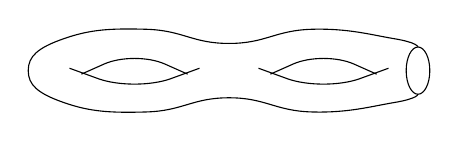
\begin{tikzpicture}[scale=1.5]
      \draw plot [smooth, tension=0.8] coordinates {(1.6, 0.2) (1.4, 0.27) (0.7, 0.35) (0, 0.23) (-0.7, 0.35) (-1.4, 0.27) (-1.7, 0) (-1.4, -0.27) (-0.7, -0.35) (0, -0.23) (0.7, -0.35) (1.4, -0.27) (1.6, -0.2)};
      \draw (1.6, 0) ellipse (0.1 and 0.2);

      \foreach \x in {0.8, -0.8}{
        \begin{scope}[shift={(\x, -0.03)}]
          \path[rounded corners=12pt] (-0.45, 0)--(0, 0.2)--(0.45, 0) (-0.45, 0)--(0, -0.28)--(0.45, 0);
          \draw[rounded corners=14pt] (-0.55, 0.05)--(0, -.15)--(0.55, 0.05);
          \draw[rounded corners=12pt] (-0.45, 0)--(0, 0.2)--(0.45, 0);
        \end{scope}
      }
    \end{tikzpicture}
  \end{center}
  We then have
  \[
    \pi_1 \Sigma_2 \cong \langle a_1, b_1, a_2, b_2 \mid [a_1, b_1][a_2, b_2]\rangle.
  \]
  On the other hand, the universal cover can be thought of as the hyperbolic plane $\H^2$, as we saw in IB Geometry. % insert picture!!

  So it follows that
  \[
    \pi_1 \Sigma_2 \Sigma \qi \H^2.
  \]
\end{eg}
This gives us some concrete hold on what the group $\pi_1 \Sigma_2$ is like, since people have been thinking about the hyperbolic plane for centuries.

We now turn to proving the Scharwz--Milnor lemma.
\begin{proof}[Proof of Schwarz--Milnor lemma]
  Let $\bar{B} = \bar{B}(x, R)$ be such that $\Gamma \bar{B} = X$. This is possible since the quotient is compact.

  Let $S = \{\gamma \in \Gamma: \gamma \bar{B} \cap \bar{B} \not=\emptyset\}$. By proper discontinuity, this set is finite.

  We let
  \[
    r = \inf_{\gamma' \not \in S} d(\bar{B}, \gamma' \bar{B}).
  \]
  If we think about it, we see that in fact $r$ is the \emph{minimum} of this set, and in particular $r > 0$.

  Finally, let
  \[
    \lambda = \max_{s \in S} d(x_0, s x_0).
  \]
  We will show that $S$ generates $\Gamma$, and use the word metric given by $S$ to show that $\Gamma$ is quasi-isometric to $X$.

  We first show that $\Gamma = \langle S\rangle$. We let $\gamma \in \Gamma$ be arbitrary.

  Let $[x_0, \gamma x_0]$ be a geodesic from $x_0$ to $\gamma x_0$. Let $\ell$ be such that
  \[
    (\ell - 1)r  \leq d(x_0, \gamma x_0) < \ell r.
  \]
  Then we can divide the geodesic into $\ell$ pieces of length about $r$. We can choose $x_1, \ldots x_{\ell - 1}, x_\ell = \gamma x_0$ such that $d(x_{i - 1}, x_i) < r$.

  By assumption, we can pick $\gamma_i \in \Gamma$ such that $x_i \in \gamma_i \bar{B}$, and further we pick $\gamma_\ell = \gamma$, $\gamma_0 = e$. Now for each $i$, we know
  \[
    d(\bar{B}, \gamma_{i -1 }^{-1} \gamma_i \bar{B} = d(\gamma_{i - 1} \bar{B}, \gamma_i \bar{B}) \leq d(x_{i - 1}, x_i) < r.
  \]
  So it follows that $\gamma_{i - 1}^{-1} \gamma_i \in S$. So we have
  \[
    \gamma = \gamma_\ell = (\gamma_0^{-1} \gamma_1) (\gamma_1^{-1}\gamma_2) \cdots (\gamma_{\ell - 1}^{-1}\gamma_\ell) \in \langle S\rangle.
  \]
  This proves $\Gamma = \langle S \rangle$.

  To prove the second part, we simply note that
  \[
    r\ell - r \leq d (x_0 \gamma x_0).
  \]
  We also saw that $\ell$ is an upper bound for the word length of $\gamma$ under $S$. So we have
  \[
    r \ell_s(\gamma) - r \leq d(x_0, \gamma x_0).
  \]
  On the other hand, by definition of $\lambda$, we have
  \[
    d(x_0, \gamma x_0) \leq \lambda \ell_s(\gamma).
  \]
  So the orbit map is an orbit-embedding, and quasi-surjectivity follows from cocompactness. % explain that word
\end{proof}

The point of quasi-isometries was so that, for example, the quasi-isometry class of the Cayley graph does not depend on the choice of generator. However, should not be surprising that we can get finer and more precise information about the group if we choose a ``good'' set of generators, such as $\{1\}$ in the case of $\Z$.

More generally, the Schwarz--Milnor lemma tells us as long as $\Gamma$ acts`` nicely'' on the space $X$, it must be the case that $X \qi \Gamma$. However, we shall see that for appropriate choices of $X$, we can learn a lot about the group $\Gamma$.

\section{Free groups}
\begin{defi}[Free group]\index{free group}\index{$F(S)$}
  Let $S$ be a (usually finite) set. A group $F(S)$ with a map $S \to F(S)$ is called the \emph{free group on $S$} if it satisfies the following universal property: for any set map $S \to G$, there is a unique group homomorphism $F(S) \to G$ such that the following diagram commutes:
  \[
    \begin{tikzcd}
      S \ar[r] \ar[rd, dashed] & F(S) \ar[d]\\
      & G
    \end{tikzcd}.
  \]
  Usually, if $|S| = r$, we just write $F(S) = F_r$.\index{$F_r$}
\end{defi}
This says the functor $F: \mathbf{Sets} \to \mathbf{Grps}$ is left adjoint to the forgetful functor $U: \mathbf{Grps} \to \mathbf{Sets}$, if one likes fancy language.

This definition is good for some things, but not good for others. One thing it does well is that it is clear that $F(S)$ is unique up to isomorphism if it exists. However, it is not immediately clear that $F(S)$ exists! (unless one applies the adjoint functor theorem)

Thus, we must concretely construct a group satisfying this property, and this construction is often useful if we actually want to work with the set.

For concreteness, suppose $S = \{a_1, \ldots, a_r\}$ is a finite set. We consider a graph
\[
  X_r = 
  \begin{tikzpicture}[eqpic]
    \node [circ] {};
    \draw (0, 0) edge [out=-30, in=30, looseness=10, loop] (0, 0);
  \end{tikzpicture}
\]
The fundamental group $\pi_1 X_r$ acts on the universal covering $\tilde{X}_r$. We know $\tilde{X}_r$ is a simply connected graph, so it is a tree. Moreover, since it is a covering space of $X_r$, it is regular with degree $2r$ on each vertex. % rose with r petals

If $r = 2$, then this is our good old picture % label edges as a_1 (horizontal) and a_2 (vertical), and label basepoint as *
\begin{center}
  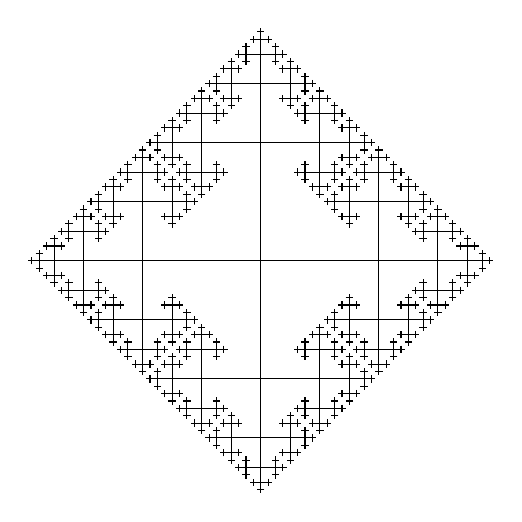
\begin{tikzpicture}[scale=0.5]
    \draw (-3, 0) -- (3, 0);
    \draw (0, -3) -- (0, 3);
    \foreach \x/\y/\rot in {3/0/0, 0/3/90, -3/0/180, 0/-3/270} {
      \begin{scope}[shift={(\x, \y)}, scale=0.5, rotate=\rot]
        \draw (0, 0) -- (3, 0);
        \draw (0, 3) -- (0, -3);
        \foreach \x/\y/\rot in {3/0/0, 0/3/90, 0/-3/270} {
          \begin{scope}[shift={(\x, \y)}, scale=0.5, rotate=\rot]
            \draw (0, 0) -- (3, 0);
            \draw (0, 3) -- (0, -3);
            \foreach \x/\y/\rot in {3/0/0, 0/3/90, 0/-3/270} {
              \begin{scope}[shift={(\x, \y)}, scale=0.5, rotate=\rot]
                \draw (0, 0) -- (3, 0);
                \draw (0, 3) -- (0, -3);
                \foreach \x/\y/\rot in {3/0/0, 0/3/90, 0/-3/270} {
                  \begin{scope}[shift={(\x, \y)}, scale=0.5, rotate=\rot]
                    \draw (0, 0) -- (3, 0);
                    \draw (0, 3) -- (0, -3);
                    \foreach \x/\y/\rot in {3/0/0, 0/3/90, 0/-3/270} {
                      \begin{scope}[shift={(\x, \y)}, scale=0.5, rotate=\rot]
                        \draw (0, 0) -- (3, 0);
                        \draw (0, 3) -- (0, -3);
                      \end{scope}
                    }
                  \end{scope}
                }
              \end{scope}
            }
          \end{scope}
        }
      \end{scope}
    }
  \end{tikzpicture}
\end{center}
We can use this to understand the fundamental group $\pi_1(X_r)$. The elements on $\pi_1 (X_r)$ are homotopy classes of based loops in $X_r$, $[\gamma]$. Using the homotopy lifting lemma, this map can be lifted to a path $\tilde{\gamma}$ in the universal cover starting at $*$.

% insert picture

Since this is a loop, we know it ends at another vertex. Because $\tilde{X}_r$ is a tree, we may homotope $\tilde{\gamma}$ rel endpoints to the unique embedded path from $*$ to the endpoint of $\tilde{\gamma}$. We can push this homotopy down to $X_r$ to get a homotopy of $\gamma$. We can see that $\gamma$ is of the following form:
\[
  \gamma = a_{i_1}^{\pm 1} a_{i_2}^{\pm 1} a_{i_3}^{\pm 1}\cdots a_{i_n}^{\pm 1}.
\]
Moreover, since $\tilde{\gamma}$ is now embedded, we know $\gamma$ is reduced, i.e.\ we never see anything looking like $a_i^{\pm 1} a_i^{\mp 1}$.

This proves a normal form theorem for elements of $\pi_1(X_r)$, namely that every element of $\pi_1(X_r)$ is represented by a unique reduced word in the generators $\{a_i\}$.

\begin{eg}
  Take the case $\pi_1 X_2 = \langle a, b\rangle$. We might be given a word
  \[
    a^3 a^6-2 b^{-2} b^3 a^5 a^{-3} a^{-3} b^{-1}.
  \]
  We can reduce this to
  \[
    a ba^{-1}b^{-1}.
  \]
  In particular, since this is not the identity, we know the original path was not null-homotopic.
\end{eg}

\begin{cor}
  $\pi_1(X_r)$ has the universal property of $F(S)$, with $S = \{a_1, \ldots, a_r\}$. So $\pi_1(X_r) \cong F_r$.
\end{cor}

\section{Finitely-presented groups}
Now if a group $\Gamma$ is generated by $S$, then we have a surjective homomorphism $F(S) \to \Gamma$. Let $K = \ker \eta$. Then
\[
  \Gamma \cong \frac{F(S)}{K}.
\]
Since we understand $F(S)$ quite explicitly, it would be nice if we have a solid gasp on $K$ as well. If $R$ normally generates $K$, so $K = \bra\bra R\ket\ket$, then we say that $\bra S \mid R \ket$ is a \term{presentation} for $\Gamma$. We will often write that
\[
  \Gamma \cong \langle S \mid R \rangle.
\]
\begin{eg}
  \[
    \Z^2 = \langle a, b\mid aba^{-1}b^{-1}\rangle
  \]
\end{eg}
Now note that if $\mathcal{P} = \langle S \mid R \rangle$ is a presentation, then we can construct as pace $X_{\mathcal{P}}$ such that $\Gamma \cong \pi_1 X_{\mathcal{P}}$, where $\Gamma \cong \bra S \mid R\ket$.

We write $S = \{a_i\}$ and $R = \{r_j\}$. We first construct a rose with $r$ petals, labeling each as one of the $a_i$. For each $j$, we glue a disk onto the rose along the path $r_j$. This is called $X_{\mathcal{P}}$.

The \term{Seifert--van Kampen theorem} tells us $\pi_1 X_{\mathcal{P}} \cong \Gamma$.

\begin{eg}
  We take the presentation $\Z^2 \cong \bra a, b \mid aba^{-1}b^{-1}\ket$. If we think hard enough (or a bit), we see this construction gives the torus:

  % insert picture

\end{eg}

Conversely, if we are given a connected cell complex $X$, we can choose a maximal tree in $X^{(1)}$, and the edges $S = \{a_i\}$ not in the maximal tree define a generating set for $\pi_1 X^{(1)}$. The attaching maps of the $2$-cells in $X$ define elements $R = \{r_j\}$ of $\pi_1 X^{(1)}$, and these data define a presentation $\mathcal{P}_X = \bra S \mid R\ket$ for $\pi_1 X$.

This is not canonical, since we have to pick a maximal tree, but let's not worry too much about that. The point of maximal trees is to get around the problem that we might have more than one vertex.

\begin{ex}
  If $X$ has one vertex, then $\Cay_S \pi_1 X = \tilde{X}^{(1)}$.
\end{ex}

\printindex
\end{document}
